\textbf{NOTE:} Empty brackets [] indicate fields where I intend to add references. \\

The cell is the basic structural component for all life on Earth. Each is comprised of a cocktail of complicated molecules that when working together enable these small units to perform their many biological functions-- often in collections, but also as individuals. Most cells must be magnified tens or hundreds of times just to be seen. How then do the constituent components of cells maneuver through their environment with only their aqueous surroundings and a slew of proteins at their disposal? As cells replicate, how do the newly copied parts find their way to opposite sides of the cell before it finally divides? 

\textbf{NOTE} Add sentence or two about focus of this thesis here.


The answer lies in part with motor proteins. Within each cell there is a vast network of interweaving protein filaments called the cytoskeleton that functions as a system of  highways to a particular class of proteins that have evolved to tackle the problem of cellular transport. These \textit{motor proteins} move along the cytoplasm by converting chemical energy into mechanical work through the hydrolysis of Adenosine triphosphate (ATP).

Why should we study motor proteins and why should this interest a physicist? To answer first question we need only consider the vast array of cellular processes in which motor proteins are critically involved. Among these include muscle contraction, axonal transprot, mitosis, meiosis, and the movement of flagella to name a few \cite{}. When motor proteins fail, these fundamental processes are jeopardized and can result in disease\cite{hirokawa_biochemical_2003}. Therefore, understanding the workings of motor proteins is vital if we are to understand how and why they fail. 

The answer to the second question is a little more complicated. Naturally, one might wonder at how such small motors can be studied in the laboratory. Kinesin and Dynein have masses of a few hundred kDa and  $\sim2$ MDa respectively \cite{liao_kinesin_1998, johnson_structure_1983}. Recalling that 1 Dalton (Da) corresponds to one atomic mass unit means these proteins consist of, at most, a few million atoms. This small scale poses a unique experimental challenge. One way this is approached here at OSU by Prof. Weihong Qiu's group is by attaching small fluorescent beads called fluorophores to the binding sites that motor proteins use to grab on to their cargo. Then, the individual movement of motors is tracked using total internal reflection fluorescence microscopy to produce video of the proteins in action as illustrated in figure \ref{fig:weihong tirf} from \cite{qiu_dynein_2012}. 

\begin{figure}[!hbt]
	\centering
	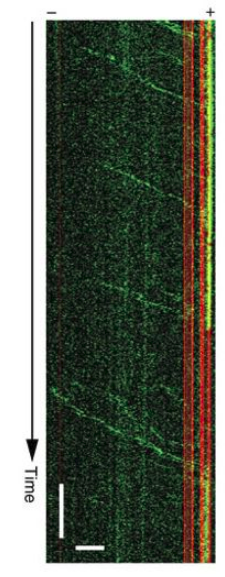
\includegraphics[width=0.25\columnwidth]{weihong_motor}
	\caption{\textbf{TIRF Microscopy Imaging} individual kinesin proteins are imaged as small green dots and tracked as they move. Slices at different times are stacked so that the slope of each green line indicates the velocity of the protein. Taken from \cite{qiu_dynein_2012}.}
	\label{fig:weihong tirf}
\end{figure}

My interest lies in how these motor proteins move as physical objects through space. Remarkably, life has evolved to make use of three primary motor proteins: myosin, kinesin, and dynein; all perform similar but slightly varied functions. This thesis is concerned specifically with dynein-- a protein unique not only for its status as the largest of the motor proteins, but also for its unique motion as drunken walker. In this thesis I continue the analysis of a proposed model for the motion of dynein along the microtublule.   
